% !TEX root = comparison.tex
\section{Experimental Setup}~\label{setup}

Two recent data analyses motivated the setup of this experiment. The first one arises from an analysis of US flight traffic data, and a finding related to how wind direction affects the efficiency of an airport.  The second one arose during the review of a paper claiming that it was impossible to statistically test for differences in center between two samples where sample size was small and from a non-normal population, with application to studying toxic waste sites. Using lineups containing dotplots we found it was possible to detect a difference, and we were curious to see if other display types (density, histogram, boxplot) might compare with dotplots.

%We want two discuss two applications, in which we are making use of lineups to compare competing designs. in the second example we are interested in visualizing mean shifts between two distributions.  

\subsection{Data Collection}
Data for both studies was collected using Amazon's Mechanical Turk (MTurk) service. 
The website for the second study is available at \url{http://www.public.iastate.edu/~mahbub/feedback_turk5/homepage.html}. Figure \ref{fig:screen} shows a screen shot of the website's layout for a dotplot lineup.

\begin{figure}[htbp] %  figure placement: here, top, bottom, or page
   \centering
   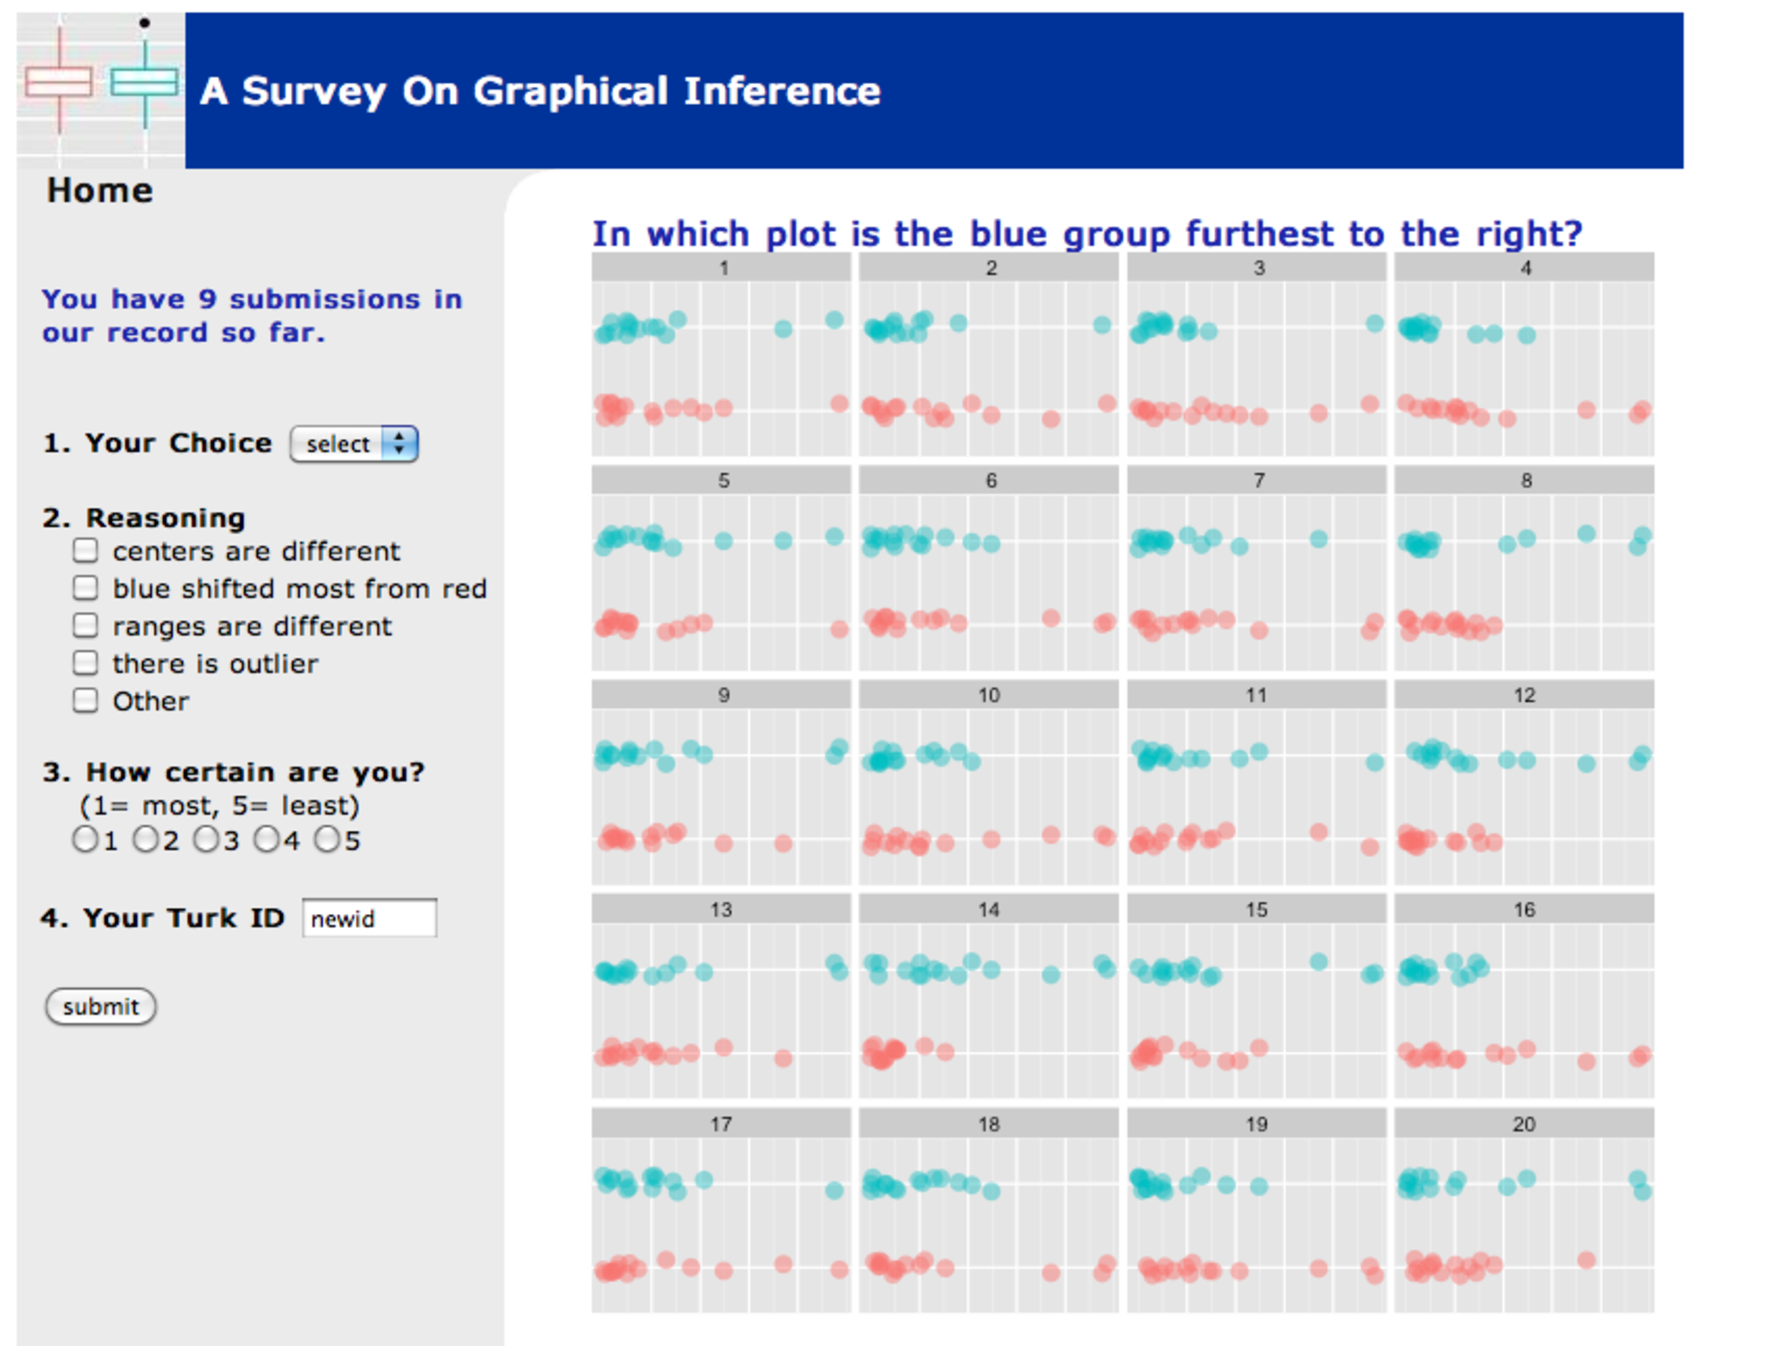
\includegraphics[width=\linewidth]{website} 
   \caption{Screenshot of the website for the second study. }
   \label{fig:screen}
\end{figure}

Each participant is shown ten lineups and asked to identify the plot that is the most different from the other plots. In the second study the `difference' is further specified as `In which plot is the blue group the furthest to the right?". 
 In both studies, though, the question is placed prominently above each lineup as a reminder of what participants are asked to look for.  Additionally, participants are asked for a reason for their choice. They can select from a list of choices particular to the lineup design, why they chose this particular plot as well as how confident they are on a scale of one to five. Personal information on age group, gender, and education is collected on a voluntary basis.  The amount of time it takes the individual to answer is also recorded.  This  allows us to assess how design choices affect decoding \cite{cleveland:1994} in terms of accuracy and speed.
 
 In order to avoid people `gaming the system' as found in earlier studies \cite{heer:2010, kosara:2010}, two of the ten lineups participants were shown were specially prepared as a baseline of performance -- if participants fail to answer some of these baseline lineups, we require at least two correct answers for the remaining plots, which is indicative of a better-than-guessing performance, as inclusion criterion for the data evaluation. 

\subsection{Wind Direction and Airport Efficiency}

The data contains all flights \cite{rita} in and out of Seattle/Tacoma International Airport (SEA) between July 2008 and June 2011. As a measure of airport efficiency we are using time between successive wheel-events (time at wheel take-off or touch-down), which we found to be independent of airline carrier and operating hours, as long as we restricted the data to `regular' operating hours between 7 am and midnight and `regular' weather conditions -- i.e. we eliminated records associated with the top 5\% wind speed measurements \cite{noaa-weather}, leaving us with just under half a million flights.

In this scenario, all of the lineups are testing the null hypothesis 

\vspace{-0.1in}
\begin{quote}
$H_0: $ {\em wind direction has no effect on efficiency }
\end{quote}
\vspace{-0.1in}

\noindent against the alternative $H_a:$ wind direction does affect efficiency.

Statistical tests of mean efficiency by wind direction are not particularly helpful in this situation: the difference in mean efficiency between the  wind direction at which the airport operates the most efficiently and its least efficient direction shows a statistically significant difference with a $p$-value $\le 10^{-15}$. %2.2e-16$.  
However, out of the 34 other wind directions,  another 31 show significant differences in efficiency as well. This is much more a property of the large data size rather than practically usable differences. Mere significances also do not allow us an assessment of the underlying pattern.

In deciding on the design for displaying efficiency by wind direction we were using the fact that wind direction is circular, and  displayed the data as (conditional) wind rose charts - i.e. for each of 36 wind directions we show the percentage of flights falling into one-minute intervals between successive flights, from  0 minutes to 8 minutes or more.

\begin{figure}[htbp] %  figure placement: here, top, bottom, or page
%   \centering
 \hspace{-.1in}
   \begin{tabular}{ccl}
   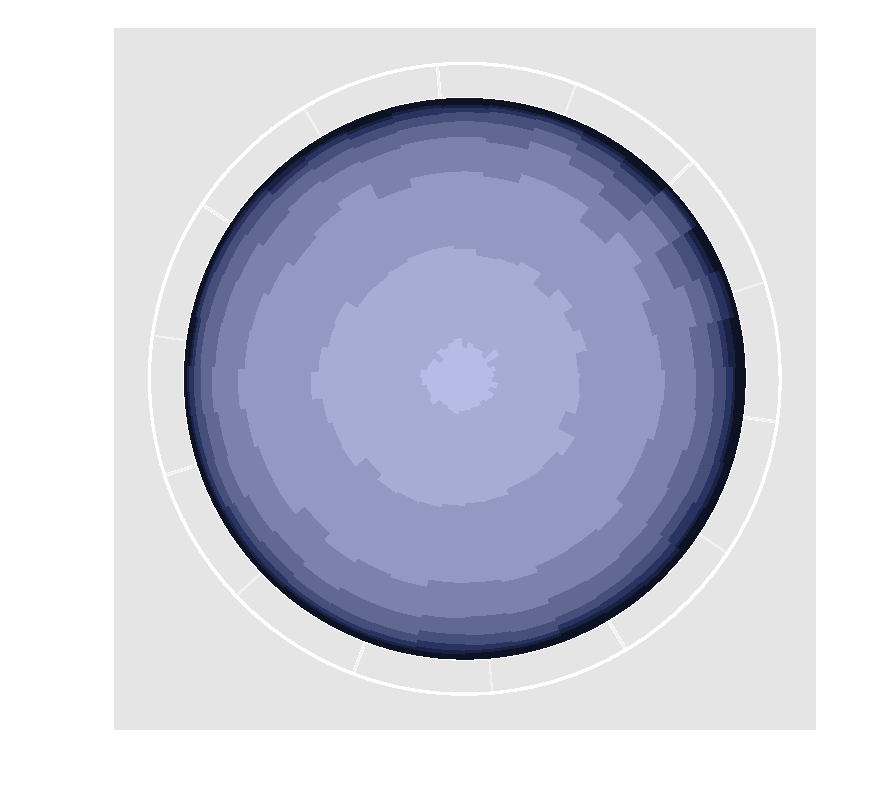
\includegraphics[width=0.43\linewidth]{Polar_NoLine.pdf} &  \hspace{-.3in}
   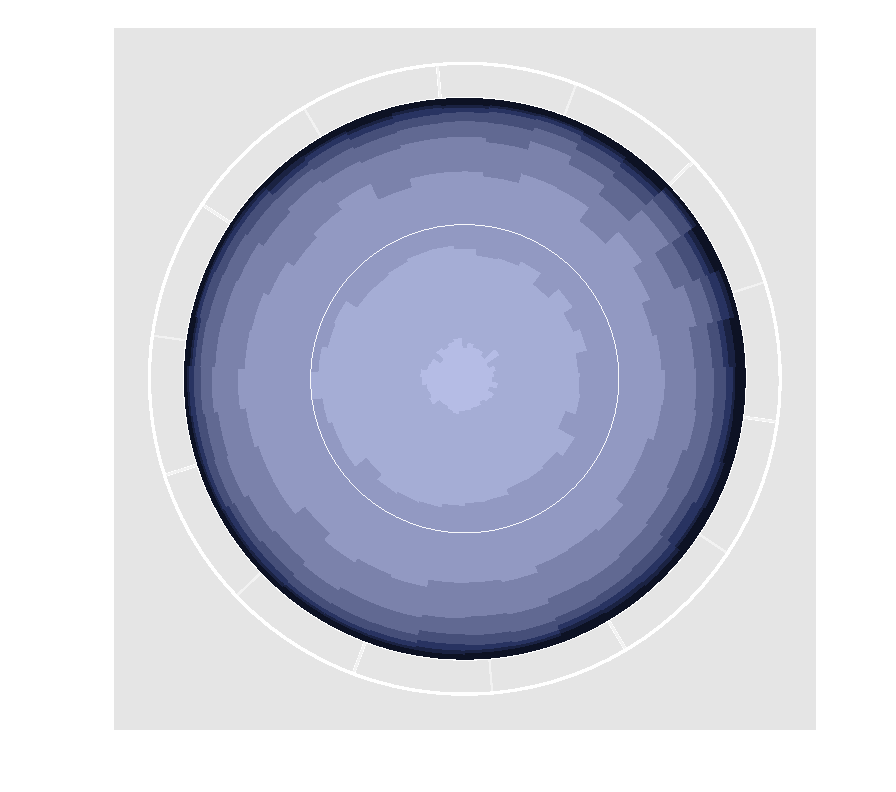
\includegraphics[width=0.43\linewidth]{Polar_Line.pdf}  &  \hspace{-.2in} \multirow{2}{*}[.55in]{  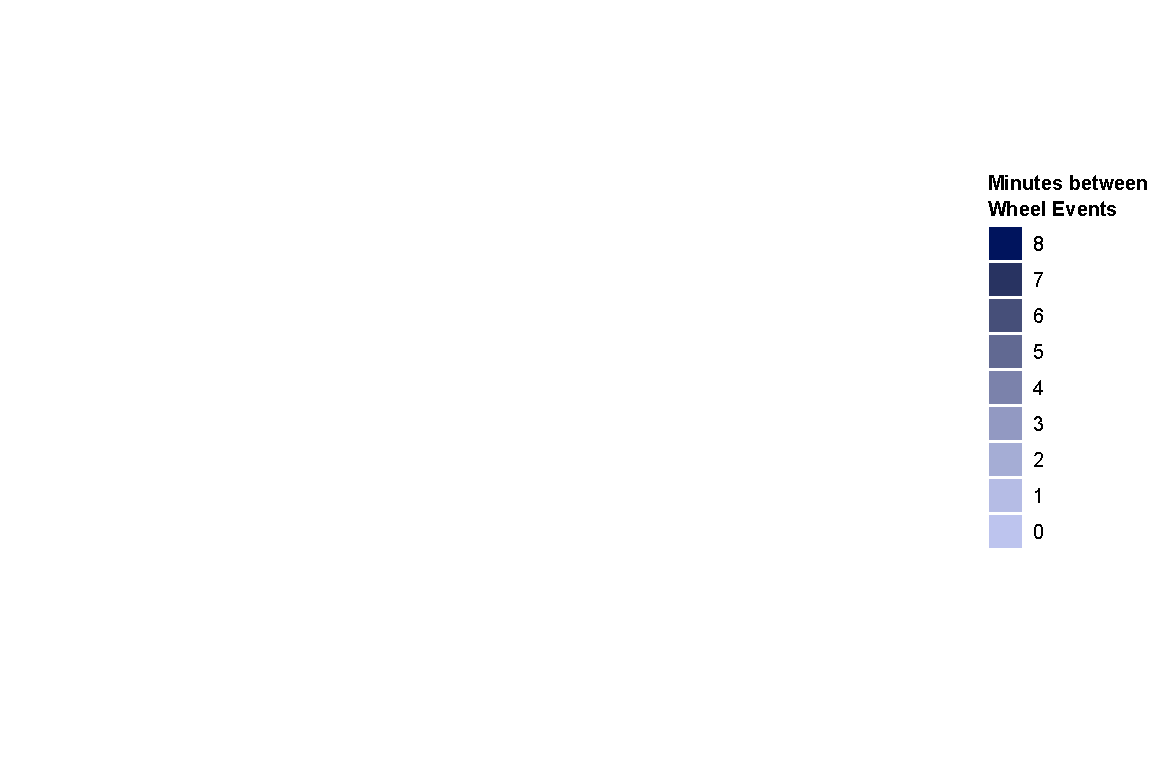
\includegraphics[width=0.2\linewidth]{legend.pdf}} \\
   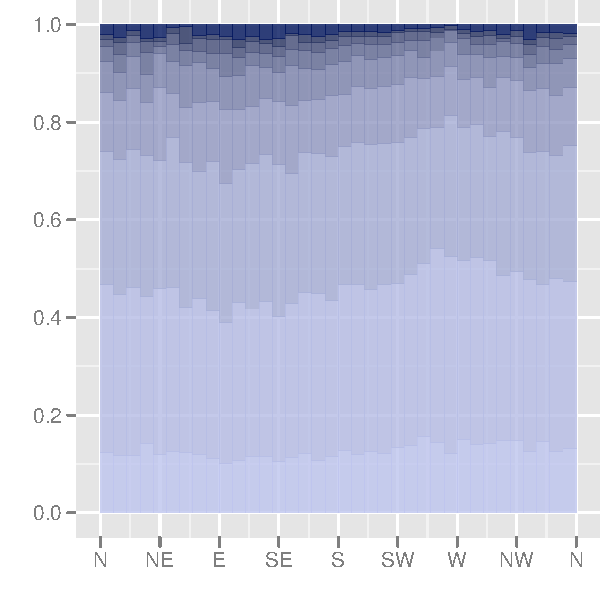
\includegraphics[width=0.375\linewidth]{euclid_noline.pdf} & \hspace{-.3in}
   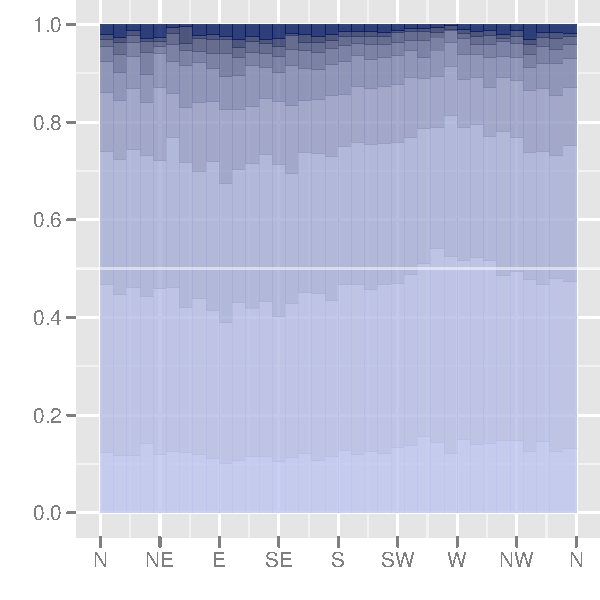
\includegraphics[width=0.375\linewidth]{euclid_line.pdf}
   \end{tabular}
   \caption{All four competing designs: polar versus Euclidean charts in top and bottom row, with (right) and without (left) reference lines at 50\%. }
   \label{layouts}
\end{figure}

In spite of the contextual circular property of wind direction, the pattern in efficiency did not seem to stand out well during the exploration process, which led us to using a corresponding  Euclidean design. Both designs were additionally equipped with a reference line at 50\%. 
Figure \ref{layouts} shows an overview of all four chart types in the study. During the exploration of the data, it became clear that Seattle airport functions at it best with winds coming from the east to southeast, while winds from the west seemed to be most troublesome, resulting in a wave-like pattern in the Euclidean charts and a shift in center for the polar charts. Since runways can be used in both directions, changing the runway usage according to dominant wind direction for that day or time of the year might be a feasible solution in gaining efficiency. 

An additional factor we were interested in this particular situation was to assess, how much of the data we actually needed to use in a design to have observers pick out the pattern. Clearly, a design is more efficient, if a smaller sample size is sufficient for showing the presence of a relationship. In order to investigate this, we took different size samples of the data and created lineup plots of all four designs for these subsets. The effect of sample size on the displays mostly stems from the additional variability introduced when using small samples, which might hide the pattern, if it is not displayed prominently. 

Another perturbation to the data are `shifts' in wind direction, i.e. we make use of the circular nature of the wind direction and adjust the $x$ axis by using different offsets.

\begin{figure}[htbp] %  figure placement: here, top, bottom, or page
   \centering
   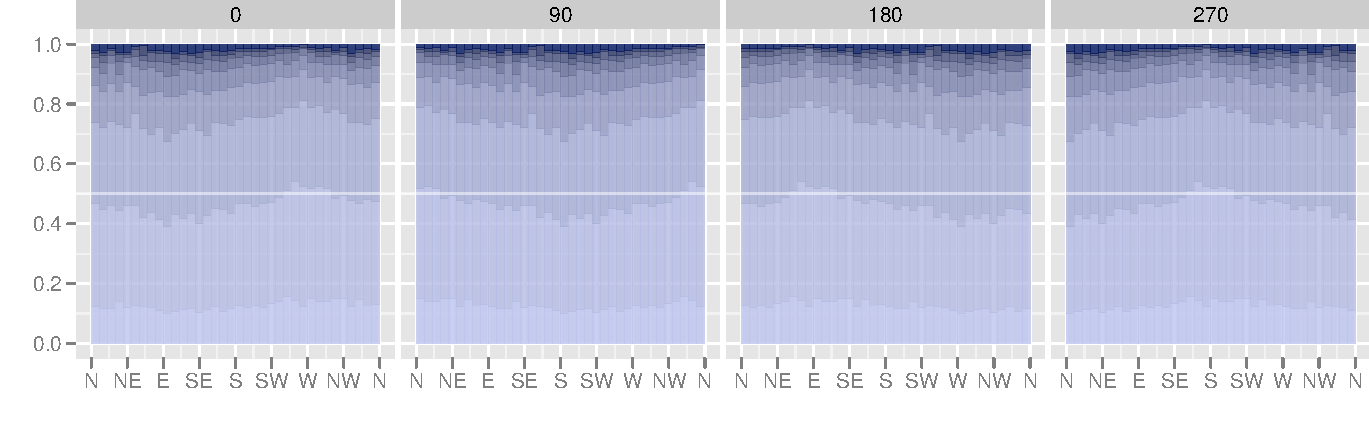
\includegraphics[width=\linewidth]{euclid-offset} 
   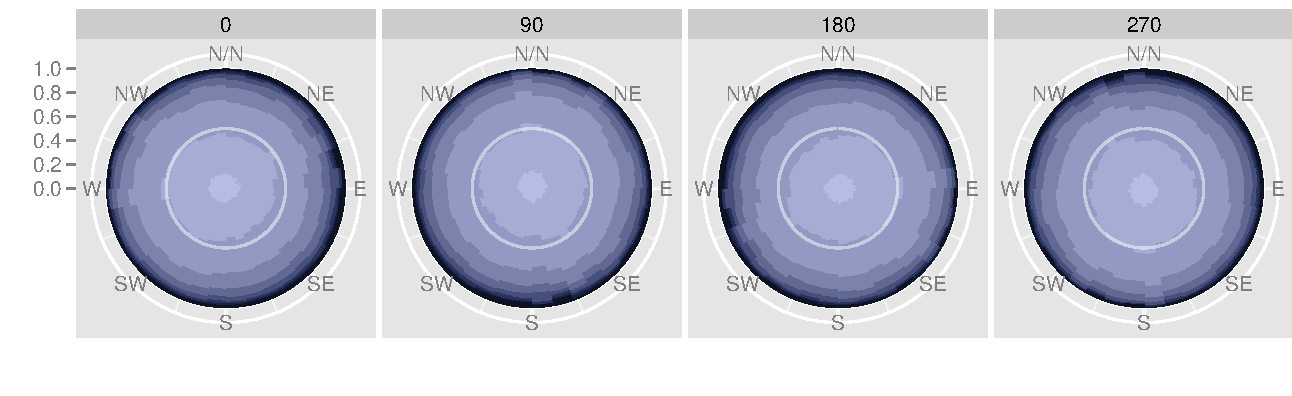
\includegraphics[width=\linewidth]{polar-offset} 
   \caption{ \label{fig:offset} (Top) Euclidean charts of the same sample, with shifts in wind direction by 90, 180, and 270 degrees. The shift by 90 and 270 leads to a `valley' versus a `mountain' pattern, whereas a shift by 180 degrees inverts the wave pattern from `down-up' to `up-down'. %\hfill\newline
      (Bottom) Shifts in wind direction in the polar chart lead to rotations of the display by 90 degrees.}
\end{figure}

 This results in a shift of the wave in Euclidean charts and a rotation in the polar charts as can be seen in Figure \ref{fig:offset}. Our initial thinking was that this would have no effect on the polar charts, but might have a deteriorating effect on the Euclidean charts, in the case that the peak or the valley of the wave was at either end of the $x$ axis, i.e. an offset of 90 or 270 degrees. 
While these simple perturbations and different sample sizes allow us to get insight into different aspects of the designs, they also allow us to get multiple responses from each observer to assess individual ability without the need to go outside the framework of the original data, i.e. we leave the joint relationship between $x$ and $y$ essentially unchanged. For all of these combinations we produced two replicates, resulting in a total of 192 different lineups ($ 4 \text{ designs} \times 6 \text{ sample sizes} \times 4 \text{ offsets} \times 2 \text{ reps})$.
Table \ref{tbl:treatment} gives an overview of the number of times lineups in each combination of design and sample size were shown, and in how many of them the data plot was correctly identified. 

\begin{table}[hbtp]
\centering
%\resizebox{\linewidth}{!} {
	%\rowcolors{1}{white}{lightgray}
	\begin{tabular}{ll@{   }r@{   }r@{   }r@{   }r@{   }r@{   }r}
	& & \multicolumn{6}{c}{sample size}  \\
        \multicolumn{2}{l}{type of chart} & 2 & 4 & 6 & 8 & 10 & 24 \\ [1pt] \hline 
	euclid & with & 12/{\bf 24}& 18/{\bf 27} & 42/{\bf 44} & 33/{\bf 41} & 39/{\bf 43} & 46/{\bf 47}\\
	       &      &(0.50)& (0.67) & (0.95) & (0.80) & (0.91) & (0.98)\\[1pt]
	& without & 13/{\bf 41} &24/{\bf 32}& 39/{\bf 44} & 47/{\bf 51} & 40/{\bf 45} & 34/{\bf 37}\\
	&         & (0.32) &(0.75)& (0.89) & (0.92) & (0.89) & (0.92)\\[3pt] %\hline
	polar & with & 13/{\bf 49}& 9/{\bf 43} & 9/{\bf 39} & 7/{\bf 35} & 8/{\bf 40} & 13/{\bf 38} \\
	      &      & (0.27)& (0.21) & (0.23) & (0.20) & (0.20) & (0.34) \\[1pt]
	& without & 6/{\bf 51}&   4/{\bf 34} &  5/{\bf 34} &  6/{\bf 39} & 11/{\bf 43} &  12/{\bf 37} \\
        &         & (0.12) & (0.12) &  (0.15) &  (0.15) & (0.26) &  (0.32)\\ 
	\end{tabular}
%	}
\caption{\label{tbl:treatment} Breakdown of lineups: number correct/\textbf{number shown} (proportion correct). Each participant was shown eight lineups, and the same lineup was shown to multiple people (denominator in the table) reasonably well-spread among the treatment levels. }
\end{table}

%Besides correctness of responses, two additional response variables were recorded:  time taken for answer and a (subjective) confidence level, ranging from 1 (lowest) to 5 (highest), assessing how convinced participants are of the correctness of their answer. 

%\begin{table}[ht]
%\begin{center}
%%\resizebox{\linewidth}{!} {
%\rowcolors{2}{white}{lightgray}
%\begin{tabular}{rrrrr}
%  \hline
% & Estimate & Std..Error & t.value & pval \\ 
%  \hline
%(Intercept) & 2.92 & 0.16 & 18.17 & 0.00 \\ 
%  polar & -0.30 & 0.16 & -1.86 & 0.06 \\ 
%  reflineTRUE & -0.16 & 0.09 & -1.74 & 0.08 \\ 
%  sample\_size & 0.01 & 0.01 & 1.01 & 0.31 \\ 
%  offset90 & 0.14 & 0.13 & 1.07 & 0.28 \\ 
%  offset180 & 0.03 & 0.13 & 0.26 & 0.80 \\ 
%  offset270 & 0.01 & 0.12 & 0.07 & 0.94 \\ 
%  polar:reflineTRUE & 0.31 & 0.13 & 2.46 & 0.01 \\ 
%  polar:sample\_size & -0.01 & 0.01 & -0.70 & 0.49 \\ 
%  polar:offset90 & -0.14 & 0.18 & -0.78 & 0.44 \\ 
%  polar:offset180 & -0.01 & 0.18 & -0.04 & 0.97 \\ 
%  polar:offset270 & -0.00 & 0.18 & -0.01 & 0.99 \\ 
%   \hline
%\end{tabular}
%%}
%\end{center}
%\caption{\label{tbl:confidence} Model output for confidence level. }
%\end{table}

%%
%%The goal of this experiment is to understand the efficiency of displaying information using euclidian and polar coordinates. Efficiency is the deviation from independence, which can be simulated by taking permutations of the original dataset. Data concerning wind patterns and time between flights at SEA airport is used for these charts. The lineup chart is composed of 20 graphics with all of the exact same characteristics except for the data. One of the 20 graphics will be using original airport data while the other 19 will be permutations of that data. Efficiency of the chart types can be inferred by how accurately individuals pick out the plot with the original data. There are other variables which are introduced to further our understanding of the way we perceive euclidian and polar coordinates. All combinations of each level of the variables are involved in the experiment for both polar and euclidian coordinates. The graphics in each chart will all have exactly the same level of the variables with the only difference being the data. 
%%
%%The other variables which are monitored are existence of reference line, placement of x-axis, and sample size. It is possible that one of the chart types benefits more from additional components such as reference lines. The polar and euclidian null charts will be shown either with or without a white reference line. The line is placed at slightly over 50 percent of the y axis. Additionally, the x-axis has four placements. The original dataset contains a characteristic wave pattern, which for euclidian coordinates, may be a large factor contributing to the perceived effectiveness of the graphic. Characteristic patterns such as the wave pattern may be perceived in a different way when viewed in polar coordinates. When the x-axis is is shifted the look of the pattern changes. The wave pattern is broken up for euclidian coordinates but for polar coordinates is only shifted around the axis. Finally, the amount of information necessary for detection as well as correctness is a measure for efficiency of the charts so the sample size which was taken from the original dataset is of interest. The original data set contained XXX,XXX observations from which 2, 4, 6, 8, 10, and 24 percent of the observations were sampled. Small sample sizes are easier to obtain because of time and money constraints. It would be nice to know if there is one type of chart which can show data trends using less information. 
%%
%%
%% All combinations of these variables were repeated for plots with a reference line and without a reference line, as shown in figure \ref{layouts}.This figure shows examples of graphics showing the actual data, which in the experiment would be randomly positioned among 19 null plots. In total there are XXX unique charts which represent all different combinations of sample size, coordinate type, x-axis placement, and whether or not there is a reference line. The charts are all assigned a difficulty level, which is based on sample size, on a scale from zero to four. There are two plots assigned a difficulty level of zero. These two charts, one polar and one Euclidian, were made from computer generated data and intended to be at the level where an individual, if he or she is not purely guessing, should be able to find the correct plot. 
%%
%%
%%Amazon's Mechanical Turk is an online service in which individuals can request and perform simple tasks and surveys for money. Using Turk we were able to gather data on how people responded to the charts. Each person is shown a series of ten charts and asked to choose the graphic on each chart which they think is "different". They then identify, from a list of choices, why they chose this particular chart as well as how confident they are on a scale of one to five. Personal information such as age group, gender, and education is also collected on a voluntary basis. The amount of time it took the individual to answer is also recorded. This study allows us to make informed judgments about how the plot type effects efficiency in terms of accuracy and time spent reading the plots. Xcite stephen few?X
%%Effect is deviation from independence. Cannot be properly measured statistically except in highly aggregated situations, where the effect might be washed out.
%%
%%Most generally this experiment can be paralleled to the pie chart versus barchart discussion. The Euclidian coordinate plot is made up of bars *whose?* areas are colored proportionally according to the data. The polar coordinate plot is made up of pie slices which are also colored proportionally according to the data. Viewers of these charts will visually decode the areas of the bars and pie slices and make a judgement based on their decoding. How accurate this judgment is is left to be discussed. According to  \cite[page=40]{kosslyn:2006}, area is usually perceived as a function of what the actual area is. This function is the area raised to an exponent of approximately 0.8 and then multiplied by a constant. However, when bars are parallel, the relative height of these bars is perceived very accurately. From this information, one could infer that the Euclidian coordinate plot may gain efficiency based on the height of the colored bars. 
%%Pie versus Barchart discussion is pretty old: cite some of the literature:
%%
%%From Stephen Few, perceptual edge:
%%	When a graph is made, quantitative and categorical information is encoded by a display method. Then the information is visually decoded. This visual perception is a vital link. No matter how clever the choice of the information, and no matter how technologically impressive the encoding, a visualization fails if the decoding fails. Some display methods lead to efficient, accurate decoding, and others lead to inefficient, inaccurate decoding. It is only through scientific study of visual perception that informed judgments can be made about display methods. (William S. Cleveland, The Elements of Graphing Data, Hobart Press, 1994, p. 1)
%%	
%%	The systematic distortion of area is captured by �Steven�s Power Law,� which states that the psychological impression is a function of the actual physical magnitude raised to an exponent (and multiplied by a scaling constant). To be precise, the perceived area is usually equal to the actual area raised to an exponent of about 0.8, times a scaling constant...In contrast, relative line length [such as the lengths of bars] is perceived almost perfectly, provided that the lines are oriented the same way \cite[page=40]{kosslyn:2006}

%%	
%%	
%%	We make angle judgments when we read a pie chart, but we don�t judge angles very well. These judgments are biased; we underestimate acute angles (angles less than 90�) and overestimate obtuse angles (angles greater than 90�). Also, angles with horizontal bisectors (when the line dividing the angle in two is horizontal) appear larger than angles with vertical bisectors. (Naomi Robbins, Creating More Effective Graphs, Wiley, 2005, p. 49)
%%	
%%	 Edward Tufte once said that �the only worse design than a pie chart is several of them, for then the viewer is asked to compare quantities located in spatial disarray both within and between pies� (Edward Tufte, The Visual Display of Quantitative Information, Graphics Press, 1983, p. 178.)
%%
%% We do not claim to settle the question - which is multi-facetted and will not have a clear 'winning' design but instead very much depends on the purpose of the chart and task at hand.

\subsection{Comparing Distribution Centers}

In a second experiment, we conducted a simulation study to investigate the power of four competing designs, as shown in Figure \ref{fig:expii}, in assessing a mean shift between distributions. The null hypothesis of each lineup is 

\vspace{-0.1in}
\begin{quote}
$H_o:$ centers of the two groups are the same,
\end{quote}
\vspace{-0.1in}

\noindent and the alternative hypothesis is $H_a:$ center of the blue group is shifted to the right.

As covariates for this experiment, we considered the {\it size of the shift}, $d$, between the means of the distributions, with $d=0.4, 0.6, 0.8. 1.0,$ and $1.2$, as well as the sample size.  Since we are dealing with two groups of points, we varied both the size of the larger group, $n_1 = 15, 45$, and 135, as well as the relative size of the second group, with $n_2 = 1/3, 2/3$ and $3/3$ of $n_1$. 
For each of these combinations, we created three replicate data sets with values from an exponential distribution with rate parameter $\lambda=1$ (for the first group) and rate parameter $\lambda_2=1/(d+1)$, which corresponds to a mean shift of $d$, for the second groups. 
Based on each data set we created four lineup charts, one for each of the competing designs. This resulted in 540 different lineup charts overall, which we sorted by $p$-value corresponding to the difference in means between the two groups in the simulated data. According to the $p$-value, we associated a `difficulty' level with lineups from 1 to 9 (easy to hard). Ten lineup plots were shown to each participant - one out of each of the difficulty levels and one additional reference chart with a particularly easy lineup  to allow for data quality checks.
\begin{figure} [hbtp]
   \centering
   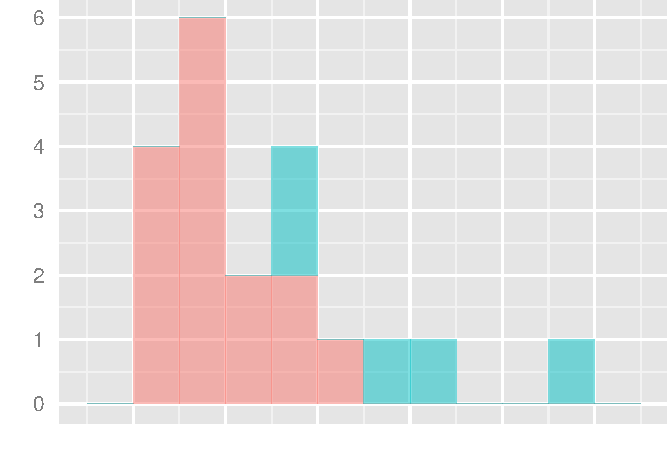
\includegraphics[width=0.45\linewidth]{hist-conc} 
   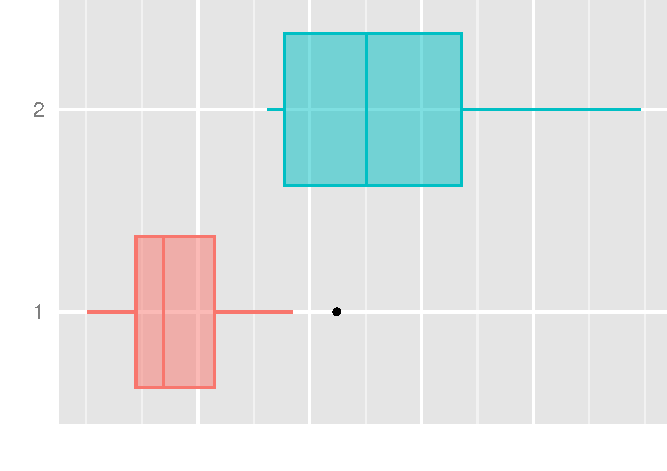
\includegraphics[width=0.45 \linewidth]{boxplot-conc} \\
   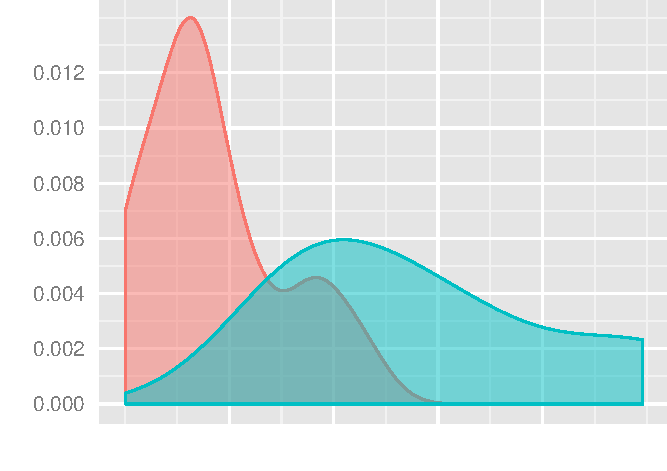
\includegraphics[width=0.45 \linewidth]{density-conc} 
   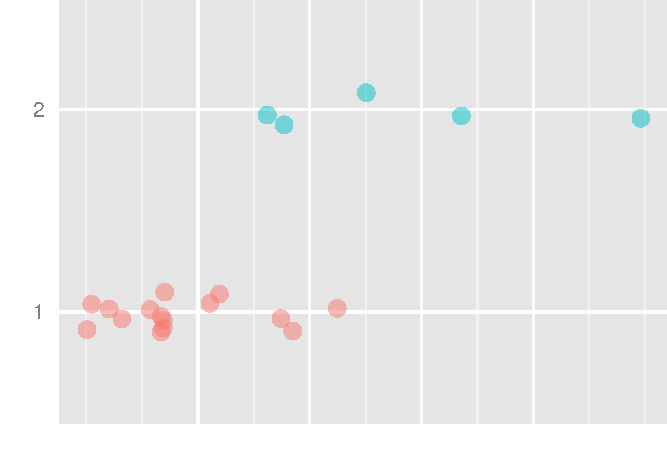
\includegraphics[width=0.45 \linewidth]{dotplot-conc} 
   \caption{Overview of all four competing designs for displaying differences in distributions.}
   \label{fig:expii}
\end{figure}
